\documentclass[a4paper,nobind]{ociamthesis}  % no extra pages
% \documentclass[a4paper,twoside,hidelinks]{ociamthesis}  % uncomment lines 99 and 100 in ociamthesis.cls
% \documentclass[a4paper]{ociamthesis}  % one-sided binding


%%% DRAFT VERSION %%%
\fancyfoot[C]{\emph{DRAFT Printed on \today}}  % draft in footer


%%% CORRECTIONS %%%
\correctionstrue  % comment out to remove corrections in blue
% \mccorrect{blah}  % word corrections
% \begin{mccorrection} ... \end{mccorrection}  % paragraph corrections


%%% BIBLIOGRAPHY %%%
\bibliographystyle{ref_style}

% uncomment for equations numbered per section rather than per chapter
% \numberwithin{equation}{subsection}


%%% TITLE PAGE %%%
\title{Diagrammatic Design of Ansätze for Quantum Chemistry}
\author{Ayman El Amrani thest}
\college{St. John's College}
\degree{Honour School of Chemistry}
\degreedate{Part II 2024}


%%% MACROS %%%
\renewcommand{\th}{\textsuperscript{th}}  % text superscripts
\newcommand{\nd}{\textsuperscript{nd}}
\renewcommand{\st}{\textsuperscript{st}}
\newcommand{\rd}{\textsuperscript{rd}}


%%% ========== BEGIN DOCUMENT ========== %%%
\begin{document}

%%% LINE SPACING CONFIG %%%
\setlength{\textbaselineskip}{26pt}  % official line spacing
\setlength{\frontmatterbaselineskip}{17pt plus1pt minus1pt} % roman pages
\setlength{\baselineskip}{\textbaselineskip}

%%% SECTION NUMBERING DEPTH CONFIG %%%
\setcounter{secnumdepth}{2}  % level that is numbered
\setcounter{tocdepth}{1}  % level that appears in table of contents


%%% ========== ROMAN PAGES ========== %%%
\begin{romanpages}
\maketitle

%%% DEDICATION %%%
\begin{dedication}
Pour ma mère et mon père. \\
Merci de m'avoir amené jusqu'ici.
\end{dedication}

%%% ACKNOWLEDGEMENTS %%%
\begin{acknowledgements}
 	Thank you Thomas Cervoni for your constant motivation and support. \\
Thank you David Tew and Stefano Gogioso for your patient supervision. \\
Thank you Razin Shaikh, Boldizsár Poór, Richie Yeung and Harny Wang for always finding the time to answer my questions. \\
Finally, thank you to all my friends and family for supporting me during this unconvential Master's.

\end{acknowledgements}

%%% SUMMARY %%%
\begin{abstract}
	A central challenge in computational quantum chemistry is the accurate simulation of fermionic systems. At the heart of these calculations lies the need to solve the Schrödinger equation to determine the many-electron wavefunction. An exact solution to this problem scales exponentially with the number of electrons. Classical computers have no means by which to efficiently store the increasingly large wavefunctions, making this problem computationally intractable in many cases. In contrast, gate-based quantum computing presents a promising solution, offering the potential to represent electronic wavefunctions with polynomially scaling resources \cite{Burton2023}. In other words, quantum computers are a natural tool of choice for simulating processes that are inherently quantum \cite{Yeung2020}.

In the last two decades, many advancements in quantum computing have been made in both hardware and software, bringing us closer to being able to simulate molecular systems. Despite these advancements, we remain in the so-called Noisy Intermediate Scale Quantum (NISQ) era, characterised by challenges such as poor qubit fidelity, low qubit connectivity and limited coherence times. The NISQ era represents a transitional phase in quantum computing, where quantum devices are not yet error-corrected but are still capable of performing computations beyond the reach of classical computers. Overcoming the limitations of the NISQ era is crucial for realising the full potential of quantum computing in various fields, including quantum chemistry and materials science.

% The Variational Quantum Eigensolver (VQE) algorithm is a method used to estimate the ground state energy of a molecular Hamiltonian by preparing a trial wavefunction, calculating its energy, and optimising the wavefunction parameters classically until the energy converges to the best approximation for the ground state energy \cite{McClean2016}. It is recognised as a leading algorithm for quantum simulation on NISQ devices due to its reduced resource requirements in terms of qubit count and coherence time \cite{Kirby2020}.

This thesis concerns itself with the study of the excitation operators used to prepare parametrised quantum circuits representing fermionic wavefunctions, known as ansätze. We extend the work of Yeung \cite{Yeung2020} on Pauli gadgets and Yordanov \textit{et al} \cite{Yordanov2020} on fermionic excitation operators, concerning ourselves with two main questions: firstly, can we use the ZX calculus to gain insights into the structure of the unitary product ansatz in the context of variational algorithms for quantum chemistry? Secondly, in the context of NISQ devices, can we use these insights to build better ansätze with reduced circuit depth and more efficient resources?

Motivated by the structure of Pauli gadgets in the ZX calculus, we began this research with the goal of identifying a general structure for the excitation operators used to prepare fermionic ansätze in the ZX calculus. We anticipated that by identifying such structures, and identifying the rules describing their behaviour, we might discover novel ways of optimising ansätze representing fermionic wavefunctions. This led us to the work done by Yordanov \textit{et al}, which shows that excitation operators can be expressed in terms of controlled-rotations. Consequently, a significant portion of this thesis revolves around developing the diagrammatic techniques essential for replicating the findings of Yordanov \textit{et al} in the ZX calculus.

\begin{itemize}
    \item \textbf{Chapter \ref{background}} develops the mathematical foundation for simulating molecules on quantum computers.
    \item \textbf{Chapter \ref{zx-calculus}} introduces the generators of the ZX calculus and its rewrite rules.
    \item \textbf{Chapter \ref{pauli-gadgets}} introduces Pauli gadgets, the basic building blocks of fermionic ansätze, and their interaction with other quantum gates.
    \item \textbf{Chapter \ref{controlled-rotations}} explores controlled rotations in terms of phase polynomials.
    \item \textbf{Chapter \ref{excitation-operators}} applies the theory developed thus far to show how excitation operators can be expressed it terms of controlled rotations in the ZX calculus.
    \item \textbf{Chapter \ref{zxfermion}} introduces the software package ZxFermion that we built, demonstrating how it can be used to replicate the research done in this thesis.
\end{itemize}

\end{abstract}

\flushbottom  % align bottom of text of each page

%%% TABLE OF CONTENTS %%%
\tableofcontents

\end{romanpages}


%%% ========== CHAPTERS  ========== %%%
\chapter{\label{intro}Introduction} 

\section{Context \& Motivation}
Example citation -- \cite{Yordanov2020}

\section{Contribution \& Thesis Structure}


\chapter{\label{background}Background}

\section{Electronic Structure Theory}
\subsection{The Hartree-Fock Approximation}
\subsection{Coupled-Cluster Theory}
\subsection{Unitary Coupled-Cluster Theory}
\subsection{Hamiltonian Simulation and Trotterisation}

\subsection{Fermionic-Qubit Encodings}
\subsubsection{Jordan-Wigner Transformation}
\subsubsection{Bravyi-Kitaev Transformation}
\subsubsection{Parity Mapping}

% \section{Quantum Computation}
% \subsection{Fundamentals}
% \subsubsection{Basis States}
% \subsubsection{Single-Qubit Statevector}
% \subsubsection{Multi-Qubit Statevector}

% \subsection{Quantum Gates}
% \subsubsection{Pauli Gates}
% \subsubsection{Rotation Gates}
% \subsubsection{Clifford Gates}

\section{The ZX Calculus}
\subsection{Generators}
\subsection{Rewrite Rules}


\chapter{\label{ch:3-variational-quantum-algorithms}Variational Quantum Algorithms}

\section{Variational Quantum Algorithms}


\chapter{\label{ch:4-phase-polynomials}Phase Polynomials}

\section{Phase Gadgets}
\subsection{Algebraic Structure}
\subsection{ZX Calculus Representation}
\subsection{Phase Gadget Decomposition}

\section{Pauli Gadgets}

\section{Controlled Rotations}



%%% ========== APPENDICIES  ========== %%%
\startappendices
\subsection{Hadamard}%
\label{appendix-hadamard}

Below are several equivalent definitions of the Hadamard generator. Note that the two rightmost definitions do not require any scalar correction.

\begin{figure}[H]
\centering
    \centering
    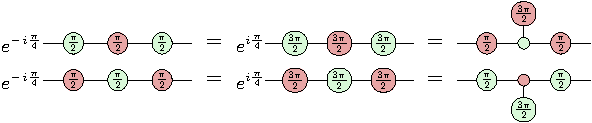
\includegraphics[width=1\textwidth]{chapter-2/hadamard_decomp}
    \caption{Equivalent definitions of the Hadamard generator.}
\end{figure}

%%%

\subsection{Phase Gadgets}%
\label{appendix-phase-gadget-fusion}

We can show how two adjacent phase gadgets fuse using the spider fusion (\ref{spider-fusion}) and bialgebra (\ref{bialgebra}) rules as follows.

\includezxdiagram{chapter-3/phase_gadget_fusion_steps}{0.8}%

%%%

\subsection{Clifford Conjugation Stuff}%
\label{conjugation}

\begin{align*}
    Ce^PC^\dagger &= C \sum_{n=0}^\infty \brac{P^n}{n!} C^\dagger \\
    CP^nC^\dagger &= \sum_{n=0}^\infty \frac{C P^n C^\dagger}{n!} \\
    CP^nC^\dagger &= \sum_{n=0}^\infty \frac{(C P C^\dagger)^n}{n!} \\
    CP^nC^\dagger &= (CPC^\dagger)^n
\end{align*}

%%%

\subsection{CNOT Commutation Relations}

\begin{figure}[H]
    \centering
    \includezxdiagram{chapter-3/cnot_commutations}{1}
    \caption{Complete set of CNOT commutation relations.}
    \label{cnot_commutations}
\end{figure}

\subsection{General One-Body Excitation Operator}%
\label{appendix-one-body-general}

\includezxdiagram{chapter-5/one_body_general_proof}{1}



%%% ========== REFERENCES ========== %%%
\setlength{\baselineskip}{0pt}

{\renewcommand*\MakeUppercase[1]{#1}%
\bibliography{references}{}

\end{document}
